\section{Double DQN}
\begin{frame}{}
    \LARGE Reinforcement Learning: \textbf{Double DQN}
\end{frame}

\begin{frame}{Double DQN}
    \begin{itemize}
        \item Q-learning suffers from a maximization bias.
        \item This is because the update target is $r + \max_a Q^\star(s,a)$. If $Q$-value is slightly overestimated then this error gets compounded.
        \pause
        \item \textbf{Solution:} Decompose the max operation in the target into action selection and action evaluation.
        \item Use the current network to select the max action for the next state and then use the target network to get the target Q-value for that action.
        \item Using these independent estimators, we can have unbiased Q-value estimates of the actions selected using the opposite estimator.
        \item We can thus avoid maximization bias by disentangling our updates from biased estimates.
    \end{itemize}
\end{frame}

\begin{frame}{DDQN Algorithm}
    \begin{figure}
        \centering
        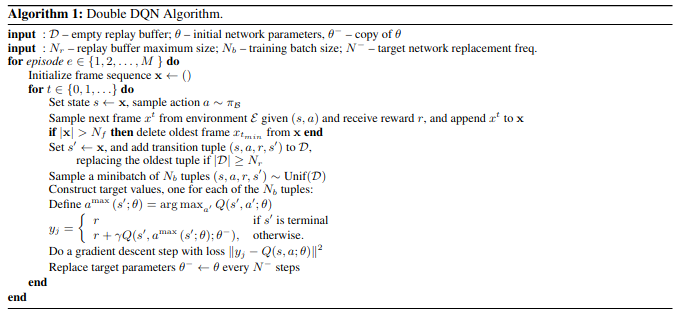
\includegraphics[width=\textwidth,height=0.9\textheight,keepaspectratio]{images/dqn+sarsa/ddqn.png}
    \end{figure}
    \footnotetext{https://leejungi.github.io/posts/Dueling-DQN/}
\end{frame}